\section{Results}


Figure~\ref{fig:benchmark-perf} and Table \ref{tab:tuned-benchmark} shows the test accuracies for each method with and without the SOT module on both datasets. 

% Without SOT:
% TM: (91.3 + 81.7 + 89.8 + 85 + 90)/5 = 87.56
% SP: (69.5 + 56.4 + 58.7 + 61.6 + 61.4)/5 = 61.52
Models without the SOT module reach an average accuracy of 87\% on the \texttt{TM} dataset and 61\% on the \texttt{SP} dataset. These results generally show that the models are capable of learning from few samples, improving significantly over the random baseline of 20\% accuracy. Furthermore, the \texttt{SP} dataset seems more challenging than the \texttt{TM} dataset. Notably, \texttt{B} outperforms all others in both datasets, whereas \texttt{B++} ranks lowest.

% With SOT:
% TM: (86.4 + 81.9 + 87.1 + 89.6 + 89.1)/5 = 86.42
% SP: (55.8 + 65.8 + 64.9 + 68 + 66.4)/5 = 64.58
Models with the SOT module yield an average accuracy of 86\% on the \texttt{TM} dataset and 65\% on the \texttt{SP} dataset, showing slight variations from non-SOT results. Performance impacts vary among methods: Meta-learners \texttt{MN}, \texttt{PT}, and \texttt{MAML} improve on \texttt{SP} with SOT, but \texttt{B}'s performance decreases. \texttt{MN}, with SOT, excels in both datasets, reaching the highest accuracy of 89\% on \texttt{TM} and 68\% on \texttt{SP}.

\textbf{Hyperparameter Ablation.} Figure~\ref{fig:hparams-swissprot-grid} shows the pair-wise interactions between all tuned hyper-parameters, methods and the inclusion of the SOT module on the \texttt{SP} data. 

% TODO: Include section about ablation of tuned hyper-parameters

\begin{figure}[h!]
    \centering
    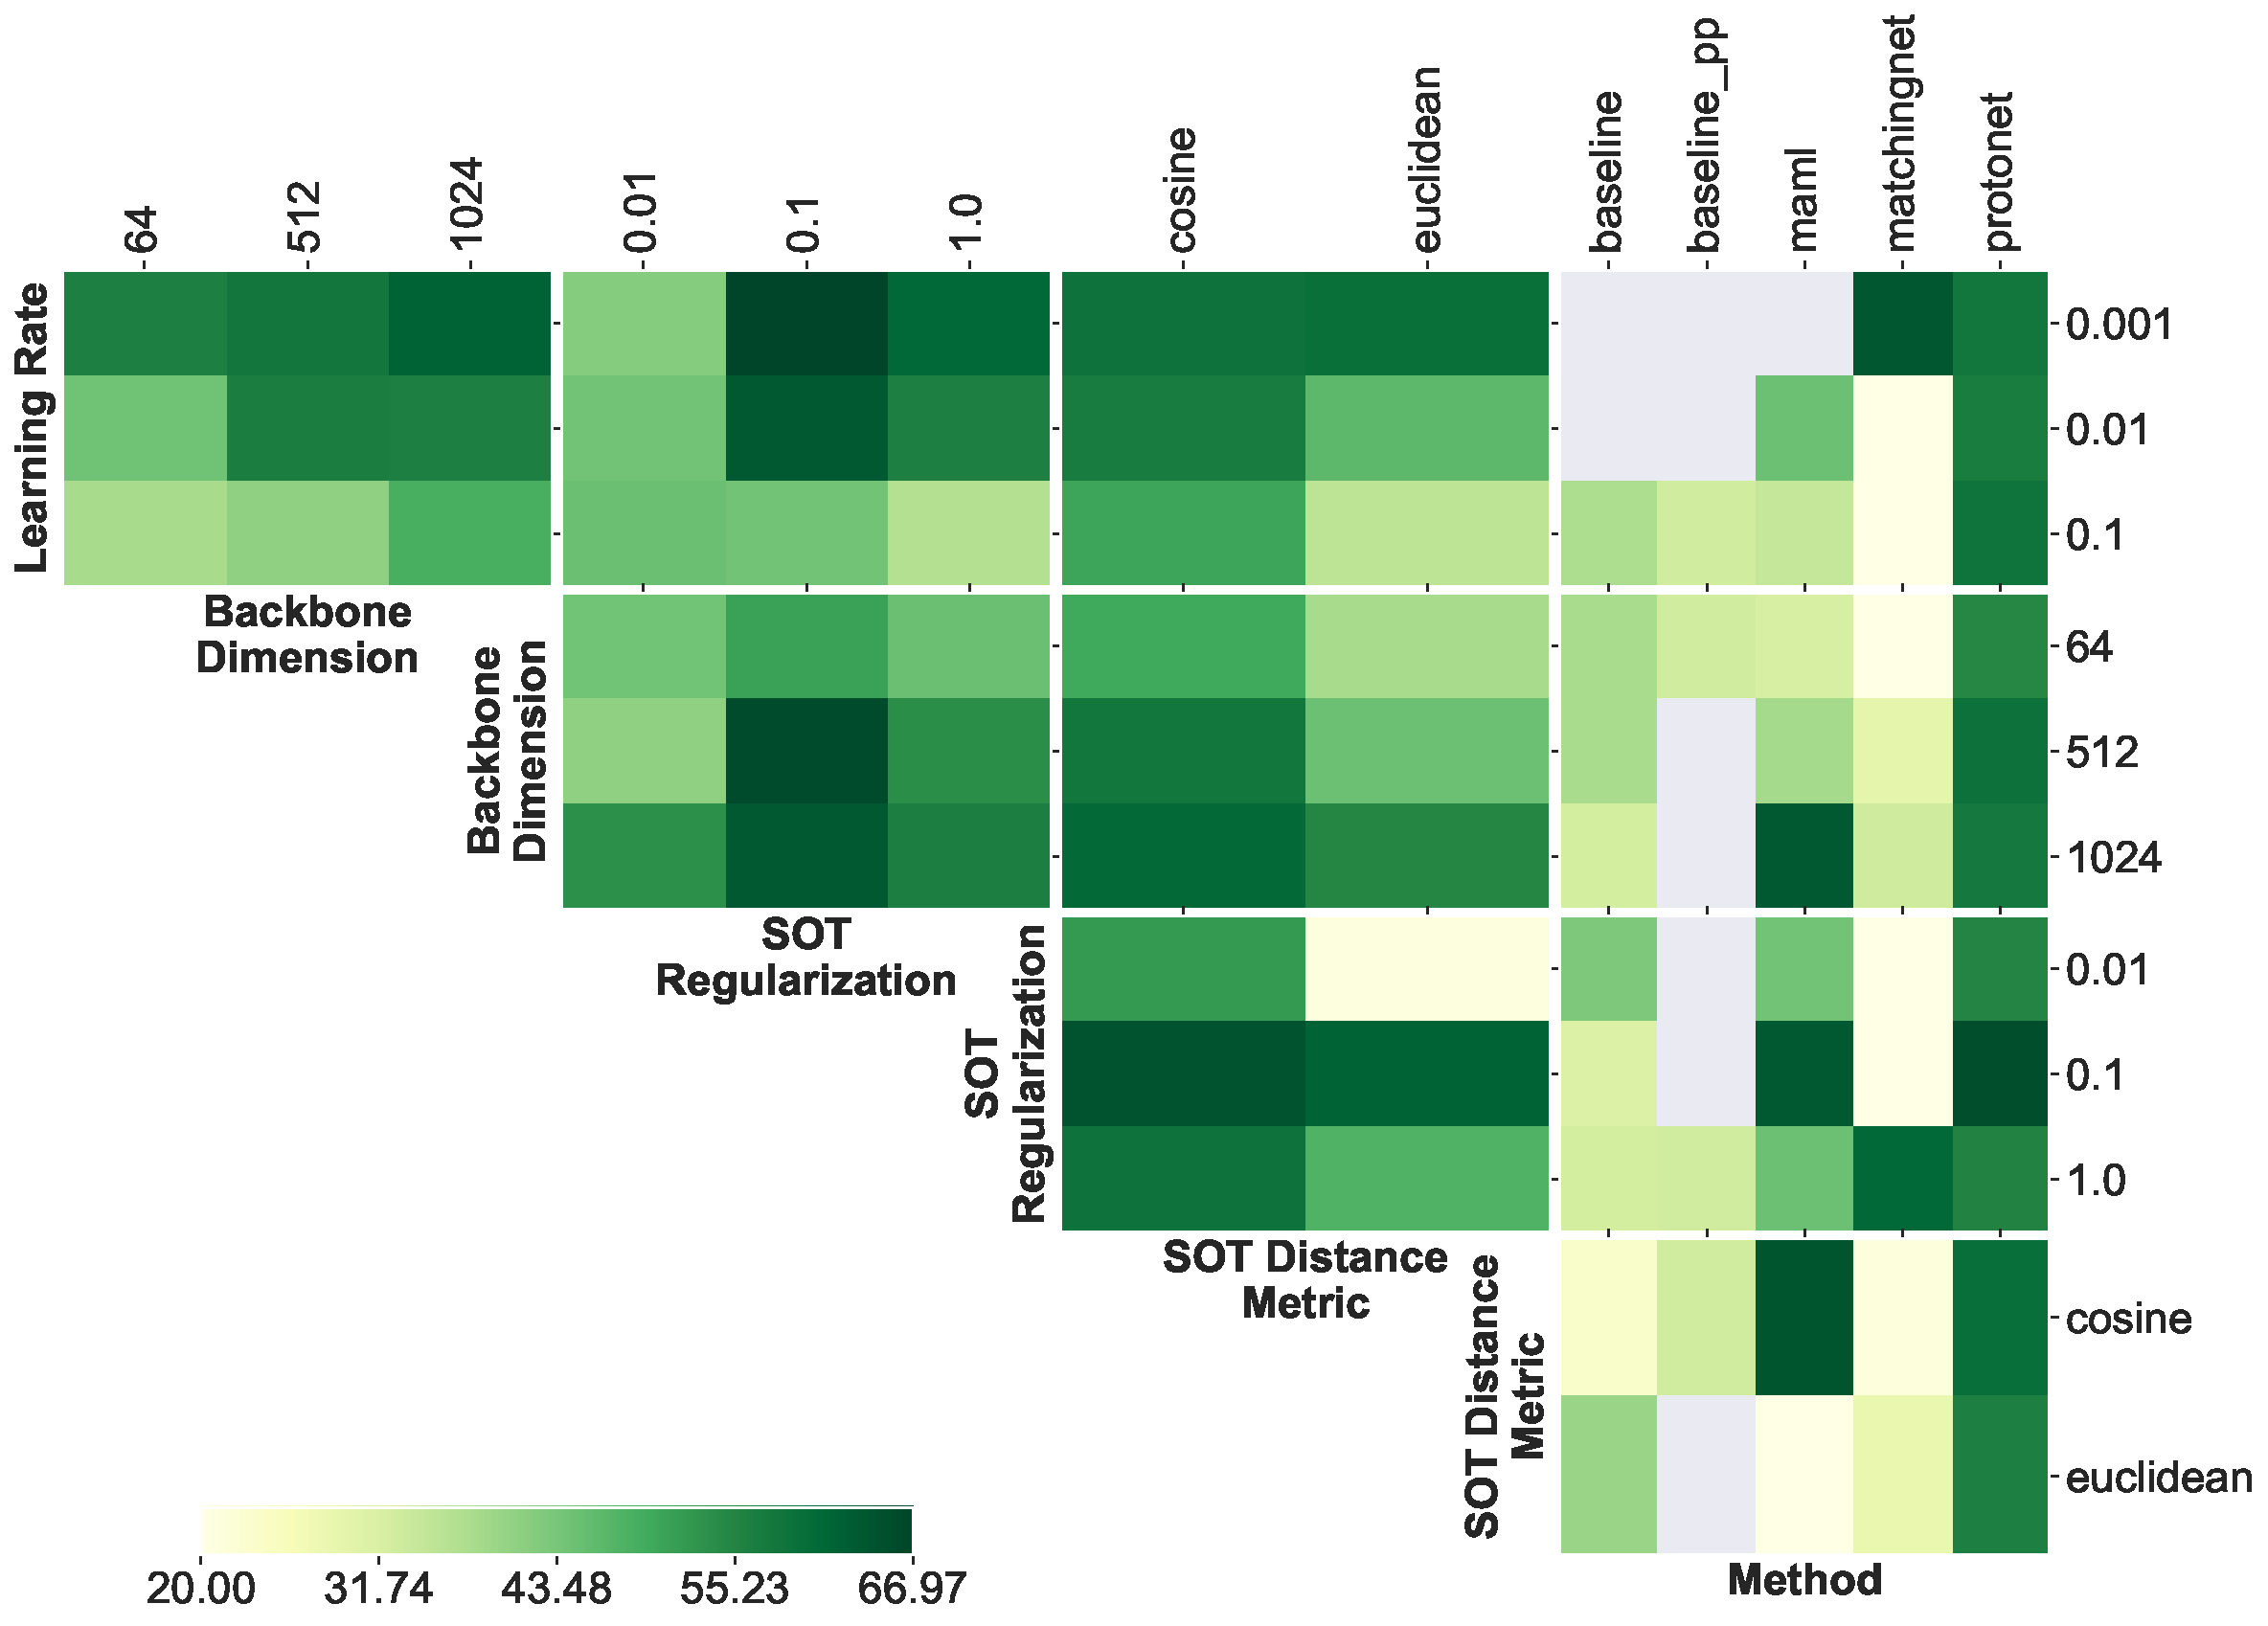
\includegraphics[width=1\columnwidth]{figures/hparams-swissprot-grid.pdf}
    \caption{\textbf{Hyperparameter Ablation.} Test accuracies on the \texttt{SP} dataset for all pairs of hyperparameter settings.}
    \label{fig:hparams-swissprot-grid}
\end{figure}

\begin{table}[ht]
\caption{
    \textbf{Benchmark Results.} Test accuracy of all methods on \texttt{TM} and \texttt{SP} in the 5-way-5-shot setting. We depict the average accuracy and the 95\% confidence interval both without (left) and with SOT (right) and the difference.
    \vspace{5pt}
}

\label{tab:tuned-benchmark}
\centering
\begin{tabular}{llllr}
\toprule
 &  & \multicolumn{2}{@{}c}{\textbf{Test Acc. (\%)}} & \\
 &  & w/o SOT & w/ SOT & Diff \\
\midrule
\multirow[c]{5}{*}{\texttt{TM}} & B & $90.7 \pm 0.7$ & $86.3 \pm 0.9$ & {\color{red} +4.8} \\
 & B++ & $81.9 \pm 0.9$ & $82.8 \pm 0.9$ &  {\color{teal} +1.1} \\
 & MAML & $\mathbf{92.8} \pm 0.5$ & $99.2 \pm 0.1$ & {\color{teal} +6.9} \\
 & MN & $84.6 \pm 0.8$ & $\mathbf{99.7} \pm 0.1$ &  {\color{teal} +17.9} \\
 & PN & $87.1 \pm 0.8$ & $98.6 \pm 0.2$ & {\color{teal} +13.2} \\
\midrule
\multirow[c]{5}{*}{\texttt{SP}} & B & $\mathbf{69.2} \pm 0.7$ & $55.7 \pm 0.8$ & {\color{red} -19.6} \\
 & B++ & $64.1 \pm 0.7$ & $64.6 \pm 0.7$ & {\color{teal} +0.8} \\
 & MAML & $68.7 \pm 0.7$ & $98.0 \pm 0.2$ & {\color{teal} +42.8} \\
 & MN & $68.2 \pm 0.8$ & $\mathbf{99.8} \pm 0.1$ & {\color{teal} +46.5} \\
 & PN & $63.5 \pm 0.7$ & $99.2 \pm 0.1$ & {\color{teal} +56.1} \\
\bottomrule
\end{tabular}
\end{table}

\textbf{Way-Shot Analysis.} Figure~\ref{fig:way-shot} illustrates \texttt{PN}'s way-shot analysis on the TM dataset, comparing scenarios with and without the SOT module. The left subplot depicts test accuracy versus the number of classes (ways), while the right subplot relates accuracy to the number of samples per class (shots). In both SOT and non-SOT contexts, a consistent trend emerges: accuracy diminishes linearly with more classes and grows concavely with additional samples per class. Notably, exceeding five samples per class yields no substantial accuracy gains. The model's performance with the SOT module is inferior for higher numbers of classes and samples.

\begin{figure}[h!]
    \centering
    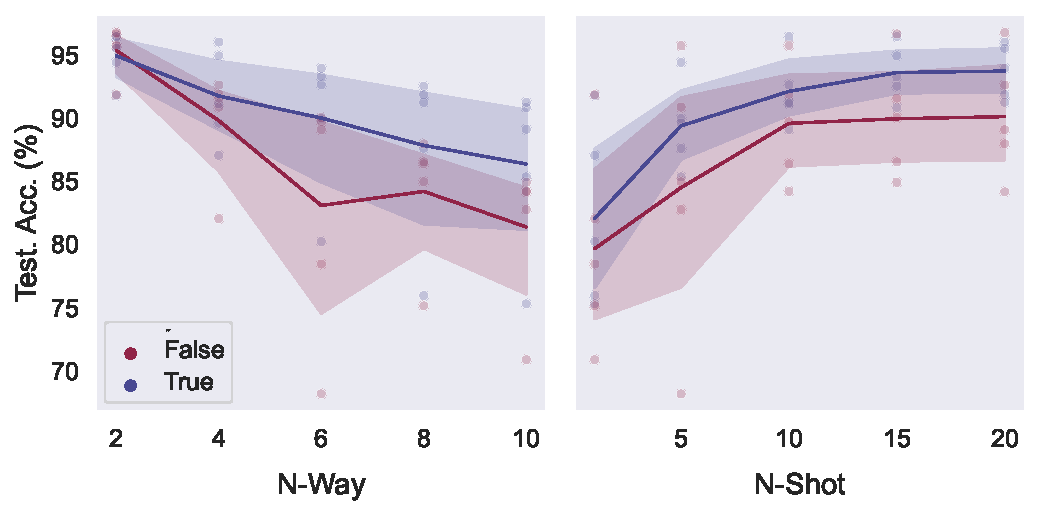
\includegraphics[width=1\columnwidth]{figures/way-shot.pdf}
    \caption{\textbf{Way-Shot Analysis.} Test accuracy of \texttt{PN} on the \texttt{TM} dataset with and without the SOT module in various 
    few-shot learning settings for fixed n-way (left) and n-shot (right). Individual points represent a single experiment. We show the regression line with a 95\% confidence interval.}
    \label{fig:way-shot}
\end{figure}
